\newpage
\section{Durchführung}
Das Experiment ist aufgebaut durch eine Kupfer-Röntgenröhre, einem LiF-Kristall und einem Geiger-Müller-Zählrohr. Diese sind in einem Gehäuse verbaut. Der LiF-Kristall kann sich um sich 
selbst rotieren. Auf einer Kreisbahn um den Kristall kann das Geiger-Müller-Zählrohr bewegt werden. Der Aufbau ist in der \autoref{fig:Aufbau} dargestellt.

\begin{figure}
    \centering
    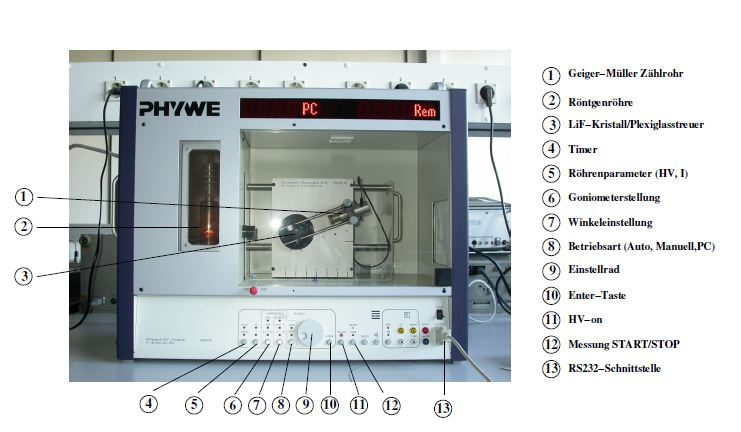
\includegraphics[height=5cm]{content/mess.JPG}
    \caption{Aufbau zur Untersuchung der Rötgenstrahlung}
    \label{fig:Aufbau}
\end{figure}

\noindent
Die Steuerung der einzelnen Elemente kann Wahlweise per Hand oder Computer erfolgen, jedoch ist es sinnvoll die unterschiedlichen Spektren mit dem Computer aufzunehmen. Die Beschleunigungsspannung
und der Emmissionsstrom werden bei allen Messungen auf $U = \SI{35}{\kilo\volt}$ und $I = \SI{1}{\milli\ampere}$ eignestellt.

\subsection{Überprüfung der Bragg Bedingung}
Um die Bragg Bedingung zu Überprüfung wird zunächst der Kristall auf einen festen Winkel $\SI{14}{\degree}$ eingestellt. Dann wird das Geiger-Müller-Zählrohr färht dann einen Winkelbereich
von von $\SI{26}{\degree}$ und $\SI{30}{\degree}$ in $\SI{0.1}{\degree}$-Schritten mit einer Integrationszeit von $\SI{5}{\second}$ pro Winkel ab.

\subsection{Emissionsspektrum der Kupfer-Röntgen-Röhre}
Um das Emissionsspektrum der Kupfer-Röntgen-Röhre zu untersuchen wird im Programm der 2:1 Koppelmodus gewählt und das Röntgenspektrum im Bereich von $\SI{4}{\degree}$ bis $\SI{26}{\degree}$
untersucht. Jedoch wurde diesmal in $\SI{0.2}{\degree}$-Schritten mit einer Integrationszeit von $\SI{5}{\second}$ gemessen.
Zusätzlich wird ein ein Detailspektrum der $K_\alpha$ und $K_\beta$-Linie gemessen. Die Einstellungen bezüglich der Messgeschwindigkeiten sind die selben wie bei der Überprüfung der Bragg Bedingung.

\subsection{Absorptionsspektren}
Nun wird um die Absorptionsspektren zu untersuchen ein Zinkabsorber vor das Geiger-Müller-Zählrohr gesetzt und das Absorptionsspektrum in $\SI{0.1}{\degree}$-Schritten gemessen. Diesmal ist
jedoch die Messzeit pro Winkel $\SI{20}{\second}$. Zusätzlich wird diese Messung für vier weitere Absorber mit Kernladungszahlen im Bereich von $30 \leq \text{Z} \leq 50$ wiederholt.



\section{Vorbereitung}
Als Vorbereitung zu dem Versuch sollte der Glanzwinkel zu verschiedenen Elementen ermittelt werden. Dieser kann mit \autoref{eqn:bragg}, den gegebenen Literaturwerten der 
K-Kante $E_\text{K}^\text{Lit}$ \cite{wissen} und der Gitterkonstante $d = \SI{201.4}{\pico\meter}$ berechnet werden mit 
\begin{equation}
    \theta_\text{glanz} = \text{arcsin}\left(\frac{h \cdot c}{E \cdot 2d}\right) \, .
    \label{eqn:theta}
\end{equation}
\noindent
Daraus folgen die Werte, die in der \autoref{tab:Glanz} aufgeführt sind. 
\begin{table}
    \centering
    \caption{Literaturwerte und daraus errechnete Größen verschiedener Elemente}
    \label{tab:Glanz}
    \sisetup{table-format=2.1}
    \begin{tabular}{c c c c c}
    \toprule
    $ $ & $Z$ & $E_\text{K}^\text{Lit} \,/\, \si{\kilo\eV}$
    & $\theta_\text{glanz}^\text{Lit} \,/\, \si{\degree}$ & 
    $\sigma_\text{k}$\\
    \midrule 
    Zn & 30 &  9,65 & 18.60042993 & 3,56 \\
    Ge & 32 & 11,10 & 16.09910447 & 3,68 \\
    Br & 35 & 13,47 & 13.20934876 & 3,85 \\
    Rb & 37 & 15,2 & 11.68329037 & 3,95 \\
    Sr & 38 & 16,10 & 11.02175704 & 4,01 \\
    Zr & 40 & 17,99 &  9.851577763 & 4,11 \\
    \bottomrule
    \end{tabular}
    \end{table}

\noindent
Zusätzlich dazu sollten die Energien bei denen die Cu-$K_\alpha$ und Cu-$K_\beta$ erwartet werden ermittelt werden. Diese liegen bei $E_{K_\alpha} = \SI{8.046}{\kilo\eV}$ und $E_{K_\beta} = \SI{8.904}{\kilo\eV}$.
Dazu lässt sich ebenfalls der Glanzwinkel jeweils bestimmen zu $\theta_{K_\alpha} = \SI{22.49}{\degree}$ und $\theta_{K_\beta} = \SI{20.22}{\degree}$.
